\documentclass{article}
\usepackage[T2A]{fontenc}
\usepackage[utf8]{inputenc}
\usepackage[russian]{babel}
\usepackage{graphicx}
\usepackage[left = 3cm, right = 2cm, top = 2cm]{geometry}
\usepackage{wrapfig}
\usepackage{amsmath}
\usepackage{float}
\graphicspath{ {./images} }
\author{Александр Романов Б01-107}
\date{}
\title{Лабораторная работа №2.1.3.\\Определение $\frac{C_p}{C_v}$ по скорости звука в газе}
\begin{document}
\maketitle

\section{Введение}

\textbf{Цель работы:} 1) измерение частоты колебаний и длины волны при
резонансе звуковых колебаний в газе, заполняющем трубу; 2) опре-
деление показателя адиабаты с помощью уравнения состояния иде-
ального газа.\\
\textbf{В работе используются:} звуковой генератор ГЗ; электронный
осциллограф ЭО; микрофон; телефон; раздвижная труба; тепло-
изолированная труба, обогреваемая водой из термостата; баллон
со сжатым углекислым газом; газгольдер.


\section{Работа}
\subsection{Установка 1}
\subsubsection{Скорость звука в воздухе}

Закачаем в первую установку воздух и будем плавно менять длину трубы, записывая значения этой длины, на которых 
произойдёт резонанс. Измерения проведём для 4 разных значений частоты. Результаты сведём в таблицу:
\begin{figure}[H]
    \centering
    \begin{tabular}{|c|c|c|c|c|}
        \hline
        \multicolumn{5}{|c|}{Воздух}                              \\\hline
        частота, kHz  & 3.00 &  3.58 & 4   & 5   \\\hline
        удлинение 1, мм & 0    &  0    & 0   & 0   \\\hline
        удлинение 2, мм & 56   &  49   & 43  & 35  \\\hline
        удлинение 3, мм & 113  &  97   & 85  & 69  \\\hline
        удлинение 4, мм &      & 145  & 128 & 106 \\\hline
        удлинение 5, мм &      & 193  & 171 & 138\\\hline
    \end{tabular}   
\end{figure}
По измеренны данным построим график удлинения трубы от номера последоготельного резонанса:

\begin{figure}[H]
    \centering
    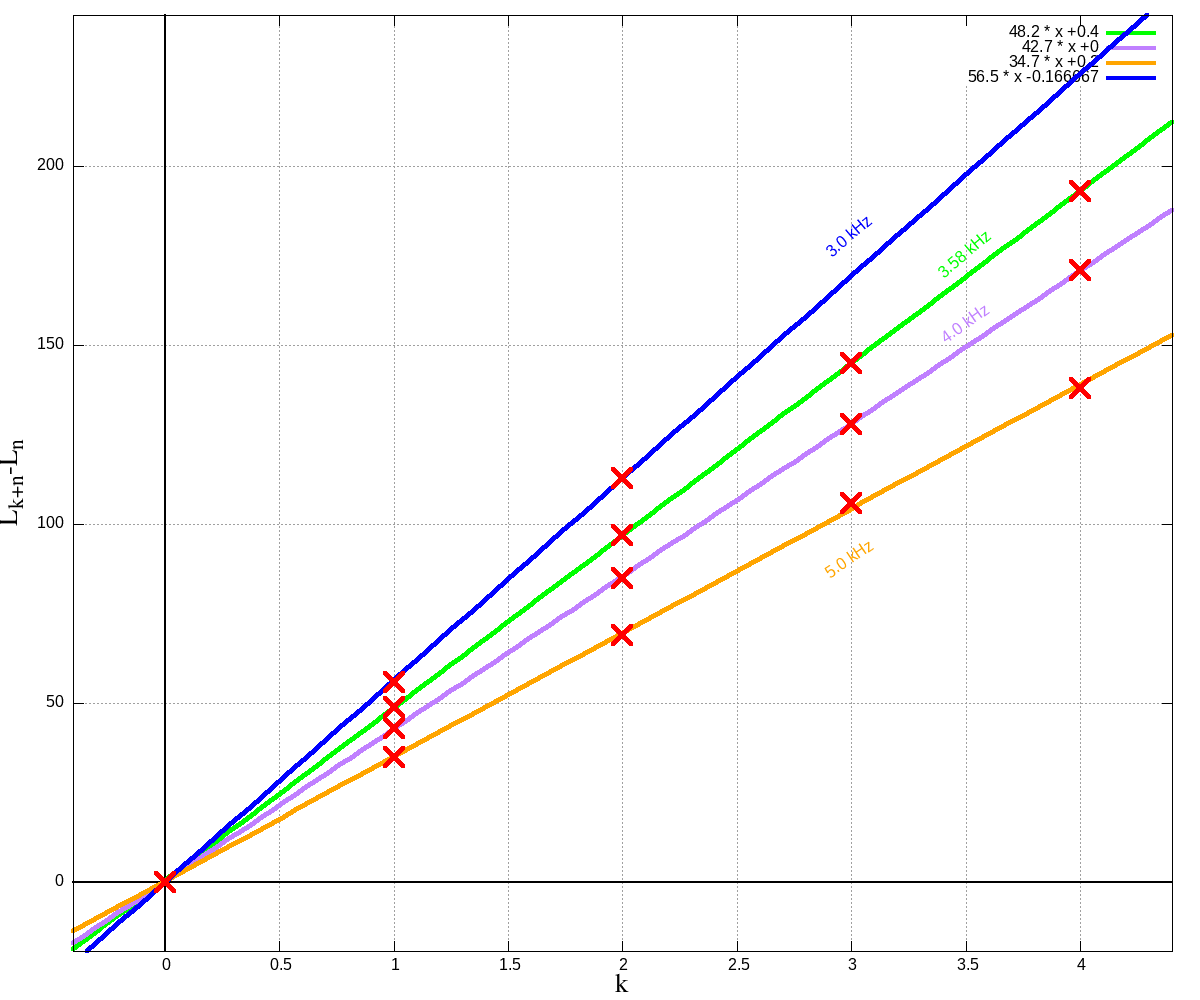
\includegraphics[width=\textwidth]{air/air.png}
    \caption{График $L_{k+n} - L_n$ от $k$ для воздуха}
\end{figure}

Отсюда по угловым коэффициентам получим значения длин полуволны:

\begin{figure}[H]
    \centering
    \begin{tabular}{|c|c|c|c|c|}
    \hline
    частота, kHz & 3.0 & 3.58 & 4.0 & 5.0 \\\hline
    $\frac{\lambda}{2}$, мм & $56.5 \pm 0.2$ & $48.2 \pm 0.1$ & $42.7 \pm 0.1$ & $34.7 \pm 1.5$ \\\hline
    \end{tabular}
\end{figure}

Согласно с формулой $c = \lambda \nu$ найдём значение скорости звука в воздухе:


\begin{figure}[H]
    \centering
    \begin{tabular}{|c|c|c|c|c|}
    \hline
    частота, kHz & 3.0 & 3.58 & 4.0 & 5.0 \\\hline
    $c$, $\frac{\text{м}}{c}$ & $339 \pm 0.6$ & $345 \pm 0.4$ & $342 \pm 0.4$ & $347 \pm 0.$\\\hline
    \end{tabular}
\end{figure}

Эти значения довольно точно совпадают с табличным ($c = 340\frac{\text{м}}{c}$). Что позволяет
говорить о неплохой точности нашего метода. А самое близкое к табличному значение получилось 
при частоте $\nu = 3.0$ kHz ($c = 339\frac{\text{м}}{c}$)

\subsubsection{Скорость звука в $CO_2$}

Проведём аналогичные измерения, заполнив трубу $CO_2$. Результаты сведём в таблицу:

\begin{figure}[H]
    \centering
    \begin{tabular}{|c|c|c|c|c|c|}
        \hline
        \multicolumn{6}{|c|}{Воздух}                      \\\hline
        частота, kHz   & 1.0 & 2,03 & 2,53 & 3,05 & 3,53  \\\hline
        удлинение 1, мм & 135 & 140  & 175  & 195  & 168  \\\hline
        удлинение 2, мм & 0   & 70   & 114  & 148  & 123  \\\hline
        удлинение 3, мм &     & 0    & 57   & 90   & 83   \\\hline
        удлинение 4, мм &     &      & 0    & 45   & 41   \\\hline
        удлинение 5, мм &     &      &      & 0    & 0    \\\hline
    \end{tabular}
\end{figure}

По эти данным построи график:

\begin{figure}[H]
    \centering
    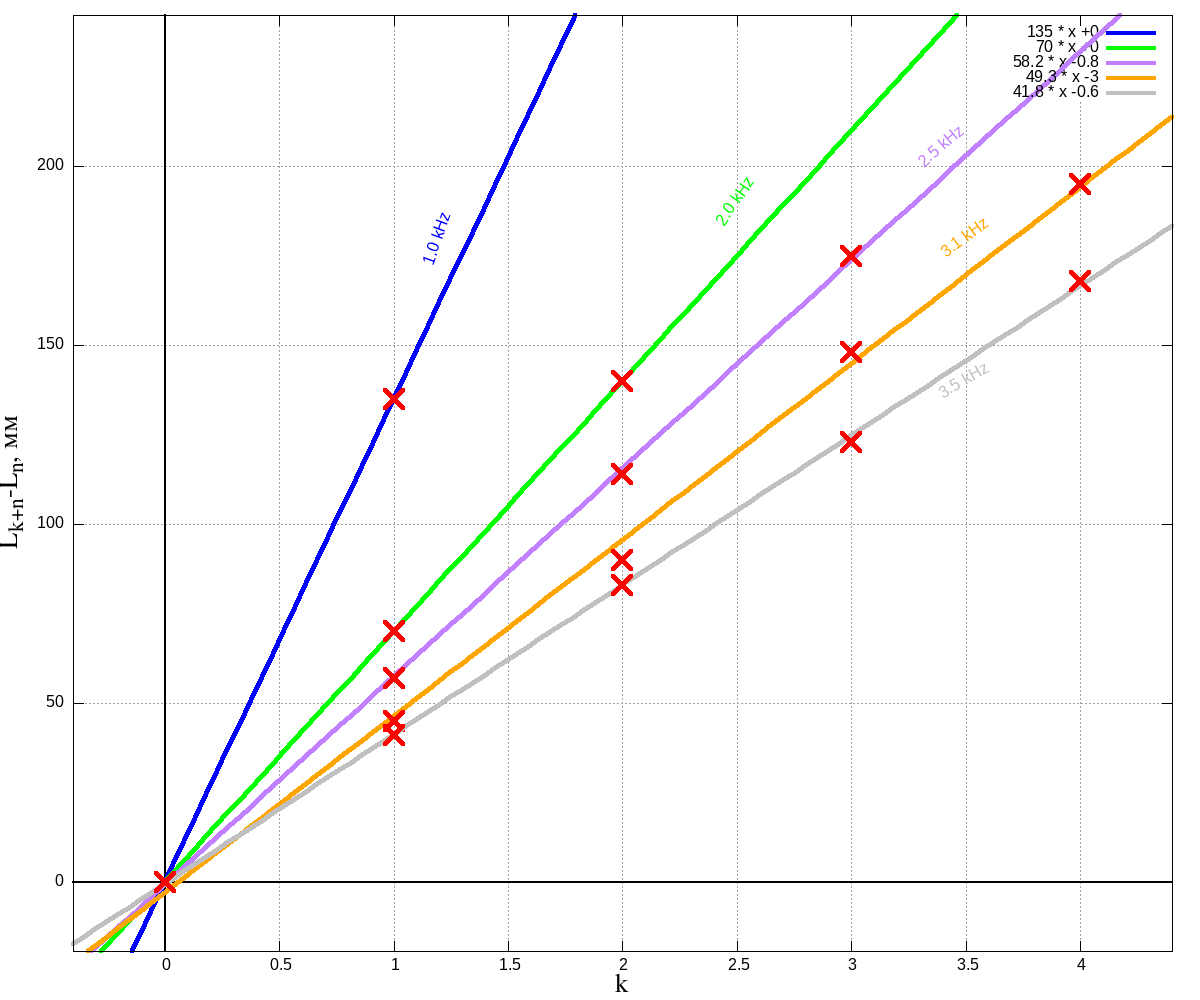
\includegraphics[width=\textwidth]{co2/co2.png}
    \caption{График $L_{k+n} - L_n$ от $k$ для $CO_2$}
\end{figure}

Отсюда по угловым коэффициентам получим значения длин полуволны:

\begin{figure}[H]
    \centering
    \begin{tabular}{|c|c|c|c|c|c|}
    \hline
    частота, kHz & 1.0 & 2.0 & 2.5 & 3.1 & 3.5 \\\hline
    $\frac{\lambda}{2}$, мм & $135 \pm 0$ & $70 \pm 0$ & $58.2 \pm 0.5$ & $49.3 \pm 1$ & $41.8 \pm 0.3$ \\\hline
    \end{tabular}
\end{figure}

Согласно с формулой $c = \lambda \nu$ найдём значение скорости звука в воздухе:


\begin{figure}[H]
    \centering
    \begin{tabular}{|c|c|c|c|c|c|}
    \hline
    частота, kHz & 1.0 & 2.0 & 2.5 & 3.0 & 3.5 \\\hline
    $c$, $\frac{\text{м}}{c}$ & $270 \pm 0$ & $280 \pm 0$ & $291 \pm 1.25$ & $296 \pm 3.1$ & $293 \pm 1.1$ \\\hline
    \end{tabular}
\end{figure}
Эти значения также достаточно точно совпадают с табличными ($c = 269 \frac{\text{м}}{c}$).
Наиболее точное значение снова выщло при наименьшей частоте ($c = 270 \frac{\text{м}}{c}$ 
при $\nu = 1.0$ kHz)

\subsection{Установка 2}
Буем измерять скорость звука в трубе постоянной длины. Плавно увеличивая частоту генератора
 получим ряд последовательных резонансных значений частоты, отмечая момент резонанса.
 Результаты сведём в таблицу:

 \begin{figure}[H]
    \centering
    \begin{tabular}{|c|c|c|c|c|}
        \hline
        \multicolumn{5}{|c|}{установка 2} \\\hline
        T, K            & 297  &  308  &  315  &  323  \\\hline
        резонанс 1, kHz & 1,23 &  1,01 &  1,02 &  1,03 \\\hline
        резонанс 2, kHz & 1,48 &  1,26 &  1,27 &  1,29 \\\hline
        резонанс 3, kHz & 1,73 &  1,51 &  1,53 &  1,54 \\\hline
        резонанс 4, kHz & 1,97 &  1,76 &  1,78 &  1,8  \\\hline
        резонанс 5, kHz & 2,22 &  2,02 &  2,03 &       \\\hline
    \end{tabular}
 \end{figure}

На основе этих данных построим график $\nu_{k+n} - \nu_n$ от $k$:

\begin{figure}[H]
    \centering
    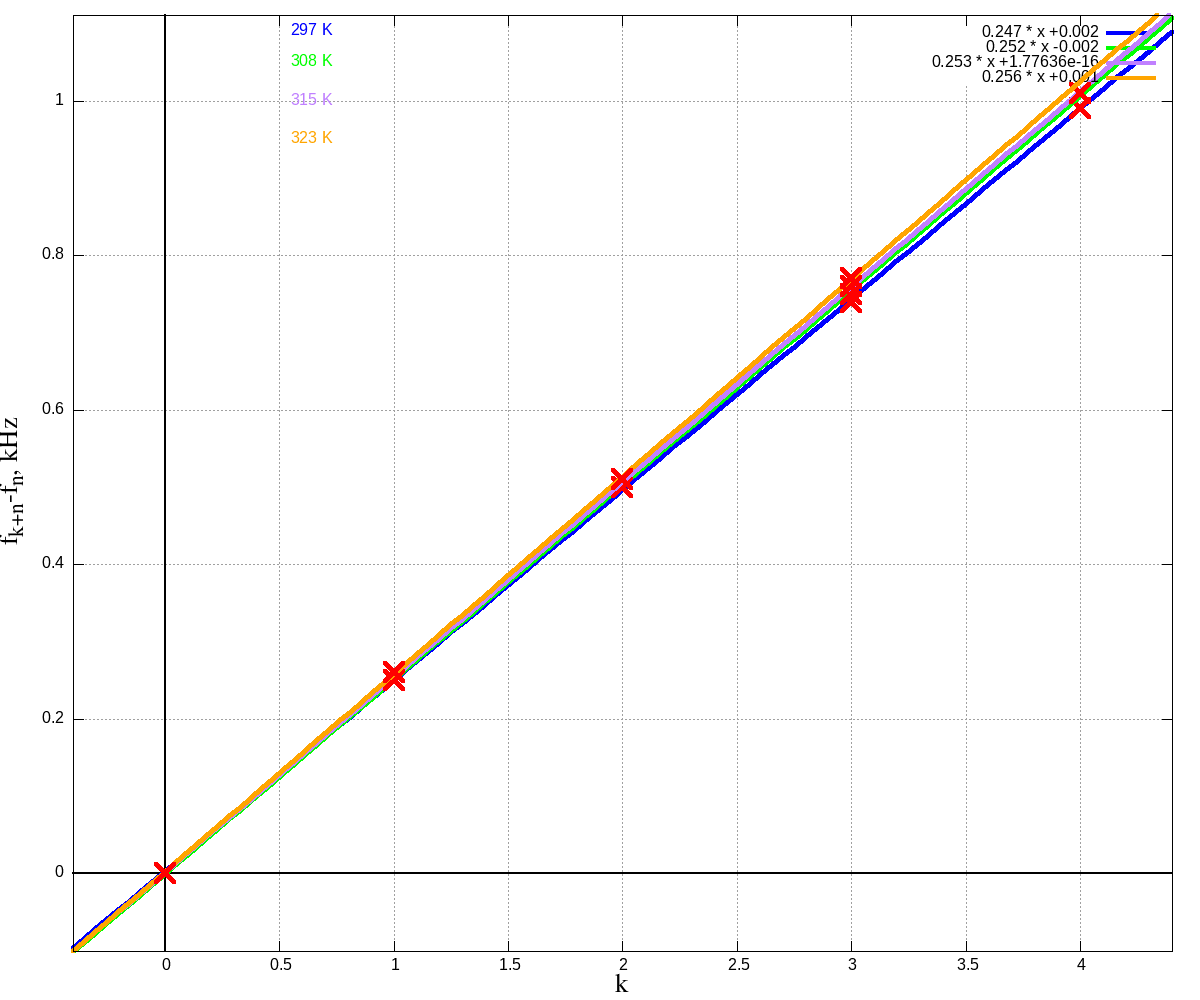
\includegraphics[width=\textwidth]{2/2.png}
    \caption{График $f_{k+n} - f_n$ от $k$ для воздуха}
\end{figure}

Зная, что длина трубы в экспериментальной установке была равна 700 мм и вспомнив формулу:

\[ f_{k+n} - f_n = \frac{c}{2L}k \]

вычислим скорости звука для каждого значения температуры:

\begin{figure}[H]
    \centering
    \begin{tabular}{|c|c|c|c|c|}
    \hline
    T, K & 297 & 308 & 315 & 323 \\\hline
    $c$, $\frac{\text{м}}{c}$ & $345 \pm 1\cdot10^{-3}$& $352 \pm 1\cdot10^{-3}$ & $354 \pm 1\cdot10^{-3}$ & $358 \pm 1\cdot10^{-3}$ \\\hline
    \end{tabular}
\end{figure}

Мы видим, что значения хорошо совпадают с теми, что были получены в первом эксперименте, и отмечаем, 
что скорость звука растётт с ростом температуры.

\subsection{Нахождение $\gamma = \frac{C_p}{C_v}$}

Вычислим отношение $\gamma = \frac{C_p}{C_v}$ по формуле:

\[ \gamma = \frac{\mu}{RT}c^2 \]
Взяв за скорость звука $c = (343 \pm 5.6) \frac{\text{м}}{c}$ из первого эксперимента, принимая $\mu_{\text{возд}} = 29 \frac{\text{г}}{\text{моль}}$ 
, а температуру в комнате за 293 K, получим:
\[ \gamma_{\text{возд}} = 1.40 \pm 5.7\cdot10^{-4}\]
Что близко к табличному значению ($\frac{7}{5} = 1.4$)

Для углекислого газа же, приняв $c = (286 \pm 13.4) \frac{\text{м}}{c}$ получим значение:
\[ \gamma_{CO_2} = 1.47 \pm 3.2\cdot 10^{-3} \]
Что близко к табличному значению ($\gamma_{CO_2} = 1.30$)
\section{Выводы}

\begin{enumerate}
    \item Итак, в нашей работе мы вычислили скорости звука в воде и углекислом газе. Они в пределах погрешности совпали с табличными,
    что говорит о хорошей точности нашего метода
    \item Измерив скорость звука при разных значениях температуры мы выяснили, что она растёт с увеличением температуры. Этот результат 
    соответствует действительности
    \item Мы использовали полученные знания о скорости звука в воздухе и углекислом газе для вычисления
    коэффициента $\gamma = \frac{C_p}{C_v}$. Коэффициенты неплохо совпали с табличными, но в случае углекислого газа всё-таки отличаются 
    больше чем на погрешность.
\end{enumerate}


\end{document}
